\section{Data Collection and Preprocessing}

\subsection{Data Collection}
%As shown by figure~\ref{fig:sysdesign}, our analysis pipeline starts from the plan, log, and system performance data collection.
%
%\stitle{Query plan parsing}
%As shown in section~\ref{sec:background}, in Hive, an execution plan is described as a text file involving hundreds to thousands of lines of operations. We parse this file first and generate a directed acyclic graph with the node as the logic vertex and the edge as the data dependencies.
%
%\stitle{Execution log and system performance processing}
%Since the Hadoop execution logs are collected with the tedious system log, we locate the records of interest by detecting the keywords from the pre-defined keyword set and then parse these logs and extract the information.
%Several important information is saved to the local file, including the task id, the logic vertices corresponding to the tasks, the temporal information(start time, duration) of tasks, the temporal information of steps in a task, etc. 

As shown in Figure~\ref{fig:sysdesign}, our visualization pipeline starts from the plan, log, and system performance data collection.

\stitle{Query plan parsing}
As introduced in Section~\ref{sec:background}, in Hive, a logical execution plan is described as a text file that contains hundreds to thousands lines of descriptions. We parse this file and generate a DAG with the vertices being the operators and the edges modeling the data dependencies.

\stitle{Execution log processing}
As Hadoop execution logs are collected from tedious system log, we locate the records of interest by first matching keywords from a pre-defined keyword set and then parsing these logs to extract the required information. The information we save to local files include task id, the logical vertex corresponding to each task, the temporal information (start time, duration) of individual tasks, and the temporal information of the sub-steps in a task. 


\subsection{Data Modeling}

\begin{figure}[t]
	\centering
	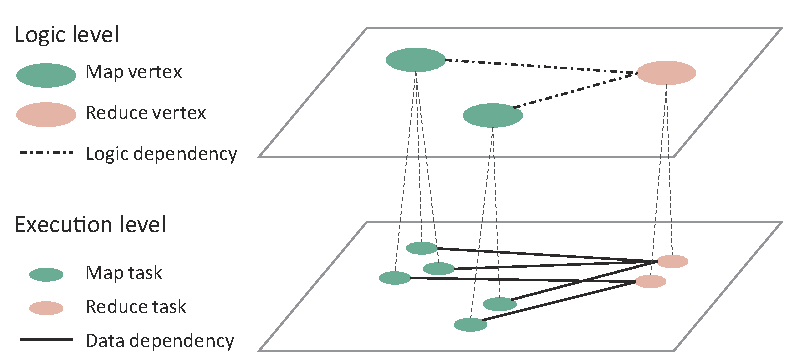
\includegraphics[width=0.42\textwidth]{figures/model/datamodel.pdf}
	\vspace{-3mm}
	\caption{Two-level execution graph.}
	\label{fig:model}
	\vspace{-3mm}
\end{figure}

The data we collected from the backend manager can be modeled as a temporal graph with two levels, i.e., the logical level and the execution-level, which is shown in Figure~\ref{fig:model}. 

%As discussed in section~\ref{sec:background}, the logic level graph indicates the DAG extracted from the execution plan, denoted by $\mathbb{G}_L = (\mathbb{V}_L, \mathbb{D}_L)$, where $\mathbb{V}_L$ is the logic vertex set and the $\mathbb{D}_L$ is logic dependency set between the vertices. The execution-level graph denotes the $\mathbb{G}_E = (\mathbb{T}_E, \mathbb{D}_E)$, where $\mathbb{T}_E$ denotes the set of tasks executed by the the physical machines and $\mathbb{D}_E$ indicates the data dependency set between tasks. 
%If a task $t \in \mathbb{T}_E$ is an physical instance of vertex $v \in \mathbb{V}_L$, we describe this relationship as the form $t \to v$. We also adopt the this description for the relationship between logic dependency $d_L \in \mathbb{D}_L$ and data dependency $d_E \in \mathbb{D}_E$ such as $d_e \to d_L$. Moreover, we use $P(v) = \{t|\forall t \to v\}$ to indicate all tasks which are the physical instances of $\mathbb{V}_L$. 
%A map task $t$ has five steps indicating as an array: $S=<s_{init}, s_{input}, s_{proc}, s_{sink}, s_{spill}>$ and a reduce task have five steps $S=<s_{init}, s_{shuffle}, s_{proc}, s_{sink}, s_{spill}>$. Each step can be modeled by a pair of attributes $<st, d>$ which denotes the start time and durzation. Notice that the different steps of the same task may have overlap in time.
%
%According to section~\ref{sec:background}, each task can be modeled as a sequence of attributes: $t:=<st, d, v, m, S_E>$, where $st$, $d$ and $v$ indicate the \textit{start time}, \textit{duration} and logic vertex of task $t$.  $m$ is the machine executes this task and $S_T$ is the corresponding steps. We use $t.attr$ to indicate the $attr$ of $t$.
%
%The vertex can be modeled as triplet: $v:=<st, d, S_L>$. The start time of $v$ is $v.st=min(\{t.st|t \in P(v)\})$, the duration of vertex $e$ is $v.d=v.st+max(\{(v.st+v.d)|t \in P(v) \})$. The steps $S_L=$ $\{d_{init}, d_{input}, d_{proc}, d_{sink}, d_{spill}\}$ or $\{d_{init}, d_{shuffle}, d_{proc}, d_{sink}, d_{spill}\}$ according to the types, and with a given $v$, $d.attr = sum(\{s.attr| s\in S_L\})$ where $attr \in \{init, input, shuffle, proc, sink, spill\}$. 

The logical level graph is the DAG extracted from the execution plan, denoted by $\mathbb{G}_L = (\mathbb{V}_L, \mathbb{D}_L)$, where $\mathbb{V}_L$ is the logical vertex set and $\mathbb{D}_L$ is logical dependency set between the vertices. The execution level graph is denoted as $\mathbb{G}_E = (\mathbb{T}_E, \mathbb{D}_E)$, where $\mathbb{T}_E$ is the set of tasks executed by the physical machines and $\mathbb{D}_E$ indicates the data dependency set between tasks. 
If a task $t \in \mathbb{T}_E$ is a physical instance of vertex $v \in \mathbb{V}_L$, we describe this relation using $t \to v$. We also apply this description to the relation between logical dependency $d_L \in \mathbb{D}_L$ and psychical dependency $d_E \in \mathbb{D}_E$ and use $d_e \to d_L$. Moreover, we use set $P(v) = \{t|\forall t \to v\}$ to indicate all tasks that are physical instances of logical operator $\mathbb{V}_L$. 
A map task $t$ has five steps and is recorded as an array $S=<s_{init}, s_{input}, s_{proc}, s_{sink}, s_{spill}>$ while a reduce task is recorded as $S=<s_{init}, s_{shuffle}, s_{proc}, s_{sink}, s_{spill}>$. Each step is associated with a pair of time $<st, d>$, which indicates its start time and duration. Note that different steps of the same task may overlap in time due to pipelining.

Each task is modeled as a sequence of attributes $t:=<st, d, v, m, S_E>$, where $st$, $d$ and $v$ indicate the \textit{start time}, \textit{duration} and logical vertex of task $t$.  $m$ is the machine that executes $t$ and $S_T$ is the corresponding steps. We use $t.attr$ to index an $attr$ of $t$. A logical vertex is modeled as a triplet $v:=<st, d, S_L>$. The start time of $v$ is $v.st=min(\{t.st|t \in P(v)\})$, the duration of vertex $v$ is $v.d=v.st+max(\{(t.st+t.d)|t \in P(v) \})$. The steps $S_L=$ $\{d_{init}, d_{input}, d_{proc}, d_{sink}, d_{spill}\}$ or $\{d_{init}, d_{shuffle}, d_{proc}, d_{sink}, d_{spill}\}$ according to the type of the vertex (i.e., map or reduce). For a given $v$, $d.attr = sum(\{s.attr| s\in S_L\})$ where $attr \in \{init, input, shuffle, proc, sink, spill\}$. 